%%%%%%%%%%%%%%%%%%%%%%%%%%%%%%%%%%%%%%%%%
% Beamer Presentation
% LaTeX Template
% Version 1.0 (10/11/12) 
%
% This template has been downloaded from:
% http://www.LaTeXTemplates.com
%
% License:
% CC BY-NC-SA 3.0 (http://creativecommons.org/licenses/by-nc-sa/3.0/)
%
%%%%%%%%%%%%%%%%%%%%%%%%%%%%%%%%%%%%%%%%%

%----------------------------------------------------------------------------------------
%	PACKAGES AND THEMES
%----------------------------------------------------------------------------------------

\documentclass{beamer}

\mode<presentation> {
%\mode<handouts> {
%\mode<article> {


% The Beamer class comes with a number of default slide themes
% which change the colors and layouts of slides. Below this is a list
% of all the themes, uncomment each in turn to see what they look like.


%\usetheme{default}
%\usetheme{AnnArbor}
%\usetheme{Antibes}
%\usetheme{Bergen}
%\usetheme{Berkeley}
%\usetheme{Berlin}
%\usetheme{Boadilla}
\usetheme{CambridgeUS}
%\usetheme{Copenhagen}
%\usetheme{Darmstadt}
%\usetheme{Dresden}
%\usetheme{Frankfurt}
%\usetheme{Goettingen}
%\usetheme{Hannover}
%\usetheme{Ilmenau}
%\usetheme{JuanLesPins}
%\usetheme{Luebeck}
%\usetheme{Madrid}
%\usetheme{Malmoe}
%\usetheme{Marburg}
%\usetheme{Montpellier}
%\usetheme{PaloAlto}
%\usetheme{Pittsburgh}
%\usetheme{Rochester}
%\usetheme{Singapore}
%\usetheme{Szeged}
%\usetheme{Warsaw}

% As well as themes, the Beamer class has a number of color themes
% for any slide theme. Uncomment each of these in turn to see how it
% changes the colors of your current slide theme.

%\usecolortheme{albatross}
\usecolortheme{beaver}
%\usecolortheme{beetle}
%\usecolortheme{crane}
%\usecolortheme{dolphin}
%\usecolortheme{dove}
%\usecolortheme{fly}
%\usecolortheme{lily}
%\usecolortheme{orchid}
%\usecolortheme{rose}
%\usecolortheme{seagull}
%\usecolortheme{seahorse}
%\usecolortheme{whale}
%\usecolortheme{wolverine}

%\setbeamertemplate{footline} % To remove the footer line in all slides uncomment this line
%\setbeamertemplate{footline}[page number] % To replace the footer line in all slides with a simple slide count uncomment this line

%\setbeamertemplate{navigation symbols}{} % To remove the navigation symbols from the bottom of all slides uncomment this line
}

\usepackage{graphicx} % Allows including images
\graphicspath{{../figures}}
\usepackage{booktabs} % Allows the use of \toprule, \midrule and \bottomrule in tables
\usepackage{amsmath, amssymb, amsthm, gensymb,mathrsfs}%,eufrak}
\usepackage{hyperref}
\usepackage{tabularx}
\usepackage{longtable}
\usepackage{makecell}
\usepackage{multicol}
\usepackage{physics}

\newcommand{\uvec}[1]{\textbf{#1}}

\newcounter{excounter}
%\renewcommand{\thefpcounter}{\thechapter.\arabic{fpcounter}}
%\renewcommand{\thefpcounter}{\thesection.\arabic{fpcounter}}
\renewcommand{\theexcounter}{\arabic{excounter}}

\newtheorem{teorema}{Teorema}[section]
\newtheorem{definicio}{Definició}[section]

\usepackage[lastexercise]{exercise}

\graphicspath{{../figures}}

%----------------------------------------------------------------------------------------
%	 TITLE PAGE
%----------------------------------------------------------------------------------------

\title[Decision Trees]{Decision Trees} % The short title appears at the bottom of every slide, the full title is only on the title page

\author{Jordi Villà i Freixa} % Your name
\institute[FCTE] % Your institution as it will appear on the bottom of every slide, may be shorthand to save space
{
Universitat de Vic - Universitat Central de Catalunya \\
Study Abroad\\ % Your institution for the title page
\medskip
\textit{jordi.villa@uvic.cat} % Your email address
}
%\date{\today} % Date, can be changed to a custom date
\date{course 2023-2024}
\logo{
\includegraphics[width=.1\textwidth]{FCTE}}
\begin{document}

\begin{frame}
\titlepage % Print the title page as the first slide
\end{frame}

\begin{frame}
\frametitle{Index} % Table of contents slide, comment this block out to remove it
\tableofcontents % Throughout your presentation, if you choose to use \section{} and \subsection{} commands, these will automatically be printed on this slide as an overview of your presentation
\end{frame}

%----------------------------------------------------------------------------------------
%	PRESENTATION SLIDES
%----------------------------------------------------------------------------------------
\begin{frame}
  \frametitle{Preliminary note}
  The material in these slides is strongly based on \cite{kroese2020}. When other materials are used, they are cited accordingly.

  Mathematical notation follows as good as it can a \href{https://ctan.math.utah.edu/ctan/tex-archive/macros/latex/contrib/mlmath/mlmath.pdf}{good practices proposal} from the Beijing Academy of Artificial Intelligence.
  \end{frame}

%\subsection{Subsection Example} % A subsection can be created just before a set of slides with a common theme to further break down your presentation into chunks

\begin{frame}{What to expect?}
  In this session we will discuss:
  \begin{itemize}
    \item Decision trees
    \item Random Forests
    \item Boosting
  \end{itemize}
\end{frame}

\section{Tree-based methods}


\begin{frame}{Tree-based methods}
\begin{itemize}
    \item Simple, intuitive and powerfiul for both regression and classification
    \item The method divides a feature space $X$ into smaller regions and fit a simple prediction function for each region.
    \begin{description}
        \item[Regression] eg, take the mean of the training responses associated with the training features that fall in the specific region
        \item[Classification] eg, take the majority vote among corresponding response variables.
    \end{description}
\end{itemize}
\end{frame}

\begin{frame}
    \begin{figure}
        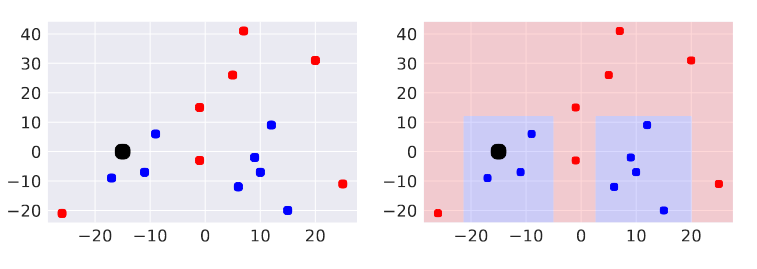
\includegraphics[width=0.9\linewidth]{F81Kroese}
        \caption{Left: training data and a new feature. Right: a partition of the feature space\cite{kroese2020}}
        \label{Fig:F81Kroese}
    \end{figure}
\end{frame}

\begin{frame}
    \begin{itemize}
        \item In the example above, we cannot separate regions linearly, but we can create rectangles in the $\mathbb{R}^2$ space.
        \item The classifier $g$, thus takes a color "blue" or "red" according to where the new black dot goes.
        \item Both the classification procedure and the partitioning can be represented by a binary {\em decision tree}.
    \end{itemize}
    \end{frame}

\begin{frame}{Partitioning of feature space $X$}
    \begin{columns}
        \begin{column}{0.4\linewidth}
            \begin{figure}
                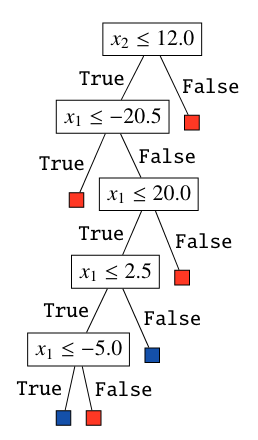
\includegraphics[width=0.7\linewidth]{F82Kroese}
                \caption{The decision tree corresponding to Fig. \ref{Fig:F81Kroese} \cite{kroese2020}.}
                \label{Fig:F82Kroese}
            \end{figure}
        \end{column}
        \begin{column}{0.6\linewidth}
           
            \begin{itemize}
                \item Each node $\nu$ corresponds to a region $\mathcal{R}_{\nu}$ of the feature space $X$. 
                \item The root node is the featre space $X$ itself.
                \item The final (undivided) leafs $w_1, w_2, \ldots$ (red/blue squares) form a partition of $X$, as they are disjoint and their union is $X$.
                \item Regional prediction functions $g^w$ are associated with each leaf.
            \end{itemize}
        \end{column}
    \end{columns}
\end{frame}

\begin{frame}{Decision}
    Let us take the input $\uvec{x}=(x_1,x_2)^T$:
    \begin{enumerate}
        \item we start at the root node, which contains a condition $x_2\leq 12.0$ that the input data satisifes;
        \item We then proceed to the left child which contains the condition $x_2 \leq -20.5$, which our data does not satisfies, so we go the next right leaf and so on.
    \end{enumerate}
    More generally, a binary tree $\mathbb{T}$ will partition the feature space into as many regions as leaf nodes, and the prediction function becomes:
    \[
        g(\uvec{x})=\sum_{w\in\mathcal{W}}g^w (\uvec{x})\mathbb{1}\{\uvec{x}\in \mathcal{R}_w\};   \quad 
        \mathscr{l}_{\tau}=\frac{1}{n}\sum_{i=1}^n \mathrm{Loss}(y_i,g(\uvec{x}_i))
    \]
    This depends on (1) how the regions $\mathcal{R}_w$ are constructed and (2) how the regional prediction functions $g^w$ of the leaf nodes are defined. $g^w$ is category in a classification setting and real-valued in regression.
\end{frame}

\begin{frame}
    \begin{Exercise}{Training loss}
        \label{Ex:trainigloss}
        Can you provide an example of the fact that any training set $\tau = \{(\uvec{x}_i,y_i),i=1,\ldots,n\}$ can be fitted via a tree with sero training loss? (Hint: imagine classifying the students in the class based on their age in days).
        \\[10pt]
        Discuss on the predictability of such model. Can you consider it overfitted?
    \end{Exercise}
\end{frame}

\section{Top down construction trees}

\begin{frame}[fragile]{Construction of the tree}
    Let us take the training set $\tau = \{(\uvec{x}_i,y_i),i=1,\ldots,n\}$. We consider the recursive algorithm:
    \begin{enumerate}
        \item First, we specify a {\em splitting rule} for each node $\nu$ (a binary 1-0 or a True-False function).
        \item Any subset of the training set can then be splitted into two sets.
        \item We can define the recursive function \texttt{ConstructSubtree} to repeat the process.
    \end{enumerate}
\end{frame}

\begin{frame}
    \label{Slide:topdown}
    \begin{figure}
        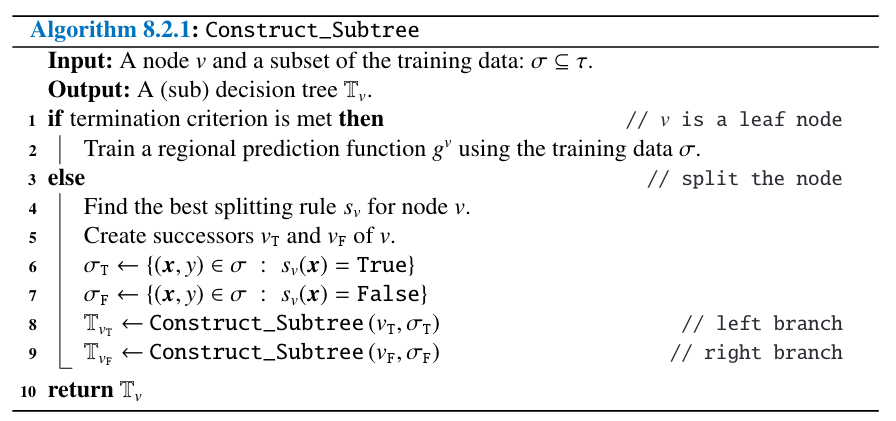
\includegraphics[width=0.7\linewidth]{A821Kroese}
    \end{figure}
    Needed tools:
    \begin{itemize}
        \item Regional prediction functions $g^{w}$
        \item Specification of the splitting rule 
        \item Termination criterion
    \end{itemize}
\end{frame}

\begin{frame}{Regional prediction functions $g^{w}$}
    
    Any function may be used for $g^{w}$ of node in a leaf $\nu=w$, but, typically:
    \begin{description}
        \item[Classification] $g^{w}$ is usually constant and equal to the most common class label of $\tau$ in the associated region $\mathcal{R}_w$
        \item[Regression] $g^{w}$ taken as the mean response in the region.
    \end{description}
\end{frame}

\begin{frame}{Splitting rules}
    
    In the algorithm in slide \ref{Slide:topdown}, we split into two subsets. For any splitting rule, the contribution to the loss is always greater if we stop the splitting at some point (see Exercise \ref{Ex:trainingloss}). So, it makes sense to {\em minimize} the training loss. 
    \begin{enumerate}
        \item[Regression] the squared-error loss of binary splitting into two child nodes $\nu_T$ and $\nu_F$  is:
        \begin{equation}
            \frac{1}{n}\sum_{(\uvec{x},y)\in\sigma_T}\mathcal{1}\{y\neq y_T^*\}+\frac{1}{n}\sum_{(\uvec{x},y)\in\sigma_F}\mathcal{1}\{y\neq y_F^*\}
            \label{Eq:squaredTLR}
        \end{equation}
        \item[Classification] the loss can be obtained from
        \begin{equation}
            \frac{1}{n}\sum_{(\uvec{x},y)\in\tau;x_j\leq \xi}(y-\bar{y}_T)^2+\frac{1}{n}\sum_{(\uvec{x},y)\in\tau;x_j\leq \xi}(y-\bar{y}_F)^2
            \label{Eq:squaredTLC}
        \end{equation}
    \end{enumerate}

    To minimize the expression \ref{Eq:squaredTL} we need to evaluate over all $j$ and $\xi$, for each of the $m\times p$ values $x_{j,k}$ and then take the minimizing pair $(j,x_{j,k})$. For \ref{Eq:squaredTLC} we can follow a similar approach.
\end{frame}

\begin{frame}{Regional prediction functions $g^{w}$}
    
    \begin{Exercise}{Splitting}
        Can you rationalize how to generate a termination criteria based on the previous fact? Post an entry in the class forum and discuss  your classmates entries.
    \end{Exercise}
\end{frame}

\begin{frame}{Measuring impurity}
    \begin{figure}
        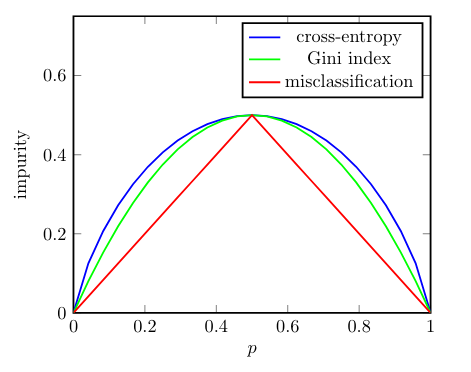
\includegraphics[width=0.6\linewidth]{F83Kroese}
        \caption{Entropy (normalized, divided by 2), Gini and missclassification impurities in binary classification (with probabilities $p$ and $1-p$). They are maximal when the label proportions are equal to $1/c$\cite{kroese2020}}
    \end{figure}
\end{frame}


\begin{frame}{Calculating information gain}
    
    \begin{Exercise}{Information gain}
        Following the description of information gain given in \href{https://towardsdatascience.com/decision-trees-explained-entropy-information-gain-gini-index-ccp-pruning-4d78070db36c}{this link}, calculate the information gain in the example given in Figures \ref{Fig:F81Kroese} and \ref{Fig:F82Kroese}. Post an entry in the class forum with the details of your calculation (either manual or computational). Discuss your classmates entries.
    \end{Exercise}

\end{frame}

\begin{frame}{Termination criterion}
    We can use a simple approach (number of data points in a tree node, for example) or when there is no advantage with more splits:
    \begin{figure}
        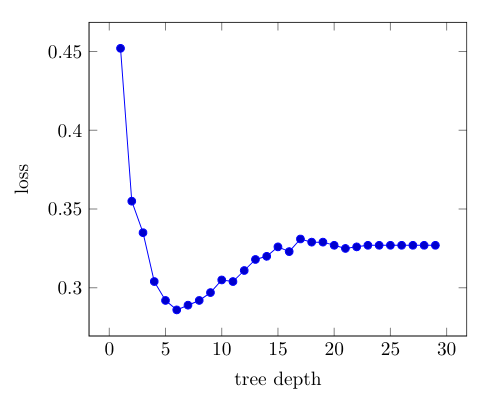
\includegraphics[width=0.7\linewidth]{F84Kroese}
        \caption{Ten-fold crossvalidation loss function as a function of the maximal {\em tree depth} in a classification problem.\cite{kroese2020}}
    \end{figure}
\end{frame}

\section{Additional considerations}

\begin{frame}
\begin{itemize}
    \item Binary (preferred) vs non binary trees. Too few data points in nodes close to the tree root.
    \item Alternative splitting rules (see Slide \ref{Slide:alternative}). Perhaps use several variables?
    \item Categorical variables ($2^k$ subsets for optimal partition with $k$ different categorical variables).
    \item Missing values (add a category of {\em missing values})
\end{itemize}
\end{frame}

\begin{frame}{Alternative splitting rules}
    \label{Slide:alternative}
    \begin{figure}
        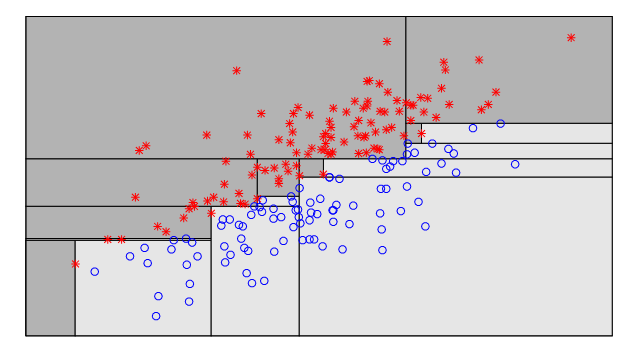
\includegraphics[width=0.9\linewidth]{F85Kroese}
        \caption{The two groups are separated, in decision tree, with a collection of rectangles, leading to an unnecessary classification procedure some times.\cite{kroese2020}}
    \end{figure}
\end{frame}

\section{Controlling the tree shape}

\begin{frame}
    \begin{figure}
        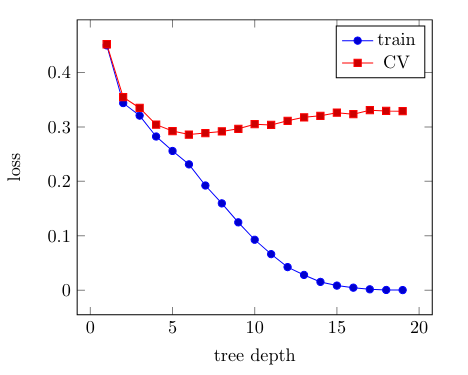
\includegraphics[width=0.7\linewidth]{F86Kroese}
        \caption{Shallow trees tend to underfit and deep trees to overfit. Cross-validation and training loss as a function of the tree depth dfor a binary classification problem.\cite{kroese2020}. Relate this plot with Exercies \ref{Ex:trainigloss}}
    \end{figure}
\end{frame}

\begin{frame}{Pruning a deep tree}
    \begin{figure}
        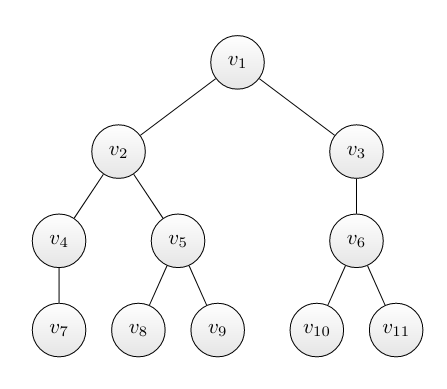
\includegraphics[width=0.7\linewidth]{F87Kroese}
        \caption{Different ancestors for different nodes.\cite{kroese2020}}
    \end{figure}
\end{frame}

\begin{frame}
    \begin{figure}{Pruning a deep tree}
        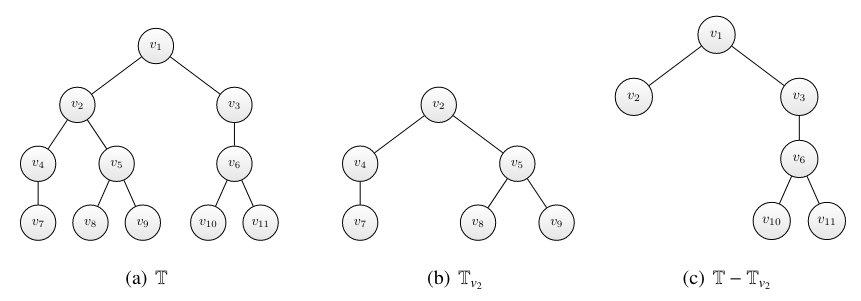
\includegraphics[width=0.9\linewidth]{F88Kroese}
        \caption{Pruning branches of the tree.\cite{kroese2020}}
    \end{figure}
\end{frame}

% \begin{frame}
%     \begin{figure}
%         \includegraphics[width=0.9\linewidth]{A841Kroese}
%     \end{figure}
% \end{frame}


\section{Boostrapping aggregation}

\begin{frame}
    \begin{figure}
        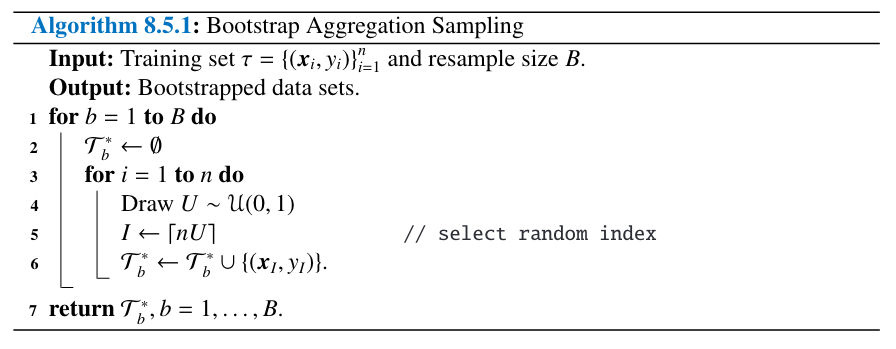
\includegraphics[width=0.9\linewidth]{A851Kroese}
    \end{figure}
\end{frame}

\begin{frame}
    \begin{figure}
        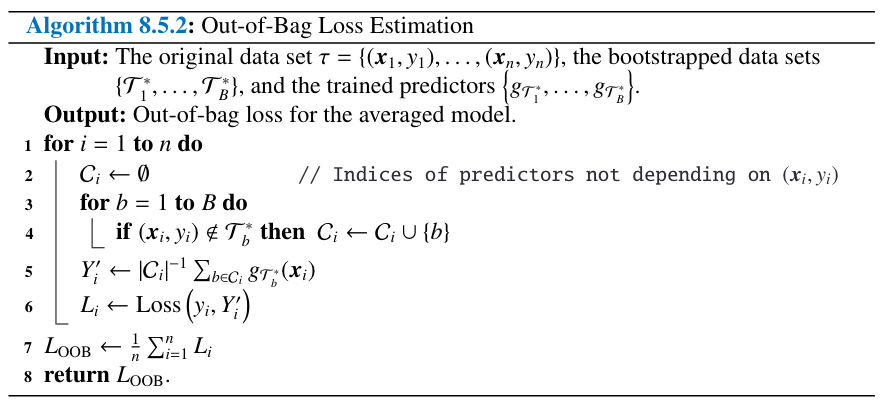
\includegraphics[width=0.9\linewidth]{A852Kroese}
    \end{figure}
\end{frame}

\section{Random Forests}

\begin{frame}
    We build a number of trees, including a subset of features in each tree construction. This way, strong predictorswill have a smaller chance to be considered at the root levels.
    \begin{figure}
        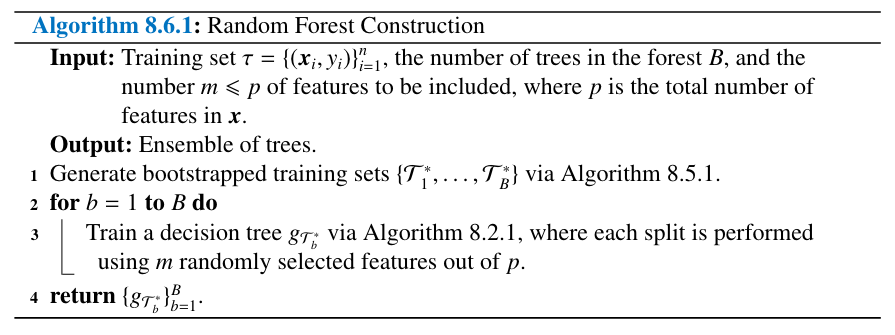
\includegraphics[width=0.9\linewidth]{A861Kroese}
    \end{figure}
\end{frame}

\begin{frame}
    \begin{figure}
        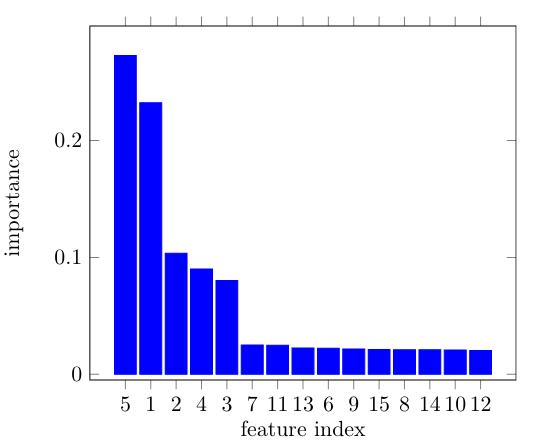
\includegraphics[width=0.7\linewidth]{F89Kroese}
        \caption{Importance measure for a 15-feature data set with only informative features $x_1,x_2,x_3,x_4,x_5$\cite{kroese2020}.}
    \end{figure}
\end{frame}

\section{Boosting}

\begin{frame}
    Similar to bootstrapping but now the predicting functions are learned sequentially, and not randomly.
    \begin{figure}
        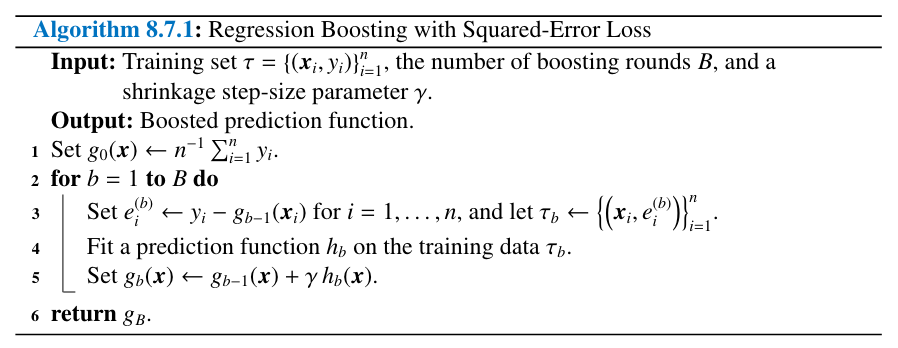
\includegraphics[width=0.9\linewidth]{A871Kroese}
        \caption{$\gamma$ controls the speed of the fitting process. For small values, boosting takes smaller steps to the training loss minimization.}
    \end{figure}
\end{frame}

\begin{frame}{Effect of $\gamma$}
    \begin{figure}
        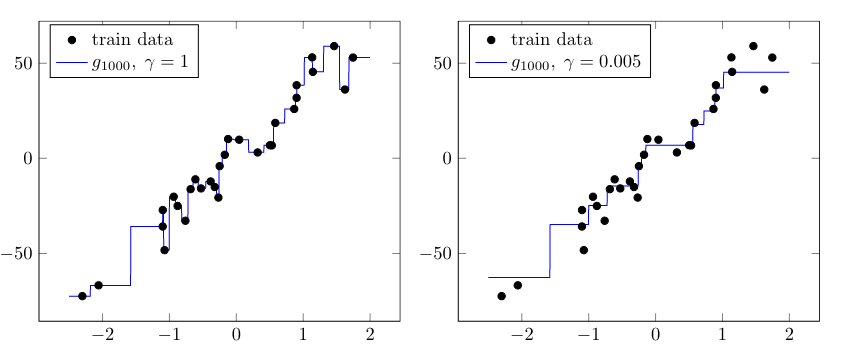
\includegraphics[width=0.9\linewidth]{F810Kroese}
        \caption{Fitted boosting regression model with two different values of $\gamma$. \cite{kroese2020}}
    \end{figure}
\end{frame}

\begin{frame}
    \begin{figure}
        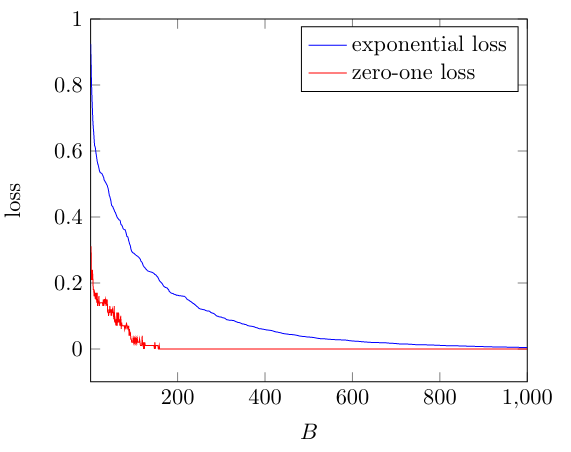
\includegraphics[width=0.7\linewidth]{F811Kroese}
        \caption{Exponential and zero-one training loss as a function of the number of boosting rounds $B$ for a binary classification problem. \cite{kroese2020}}
    \end{figure}
\end{frame}

\section{Bibliography}
\bibliographystyle{unsrt}
\bibliography{DataSciencewithPython}
\end{document}
